\documentclass{article}
\usepackage{graphicx}
\usepackage{amsmath}
\usepackage{cite}
\usepackage{color}
\usepackage{enumitem}
\usepackage{natbib}
\usepackage{tabularx}
\usepackage{natbib}
\usepackage{ragged2e}
\usepackage{geometry}
\geometry{a4paper, left=3.5 cm, right=3.5 cm, top=3 cm, bottom=3 cm}

\title{\huge\textbf{La digitalizzazione nelle PA}}
\author{\texttt{Alessandro Meloni 0001118676 GEPID}}
\date{Anno accademico 2023/2024}

\renewcommand\contentsname{Indice}
\renewcommand\refname{Bibliografia}

\begin{document}
\begin{figure}
    \centering
    
\includegraphics[width=0.9\linewidth]{Uniboarms.png}
\end{figure}
\maketitle

\centering \tableofcontents

\newpage\centering
\section{Introduzione}
\begin{justify}
L'ampliamento di tecnologie che usufruiscono di intelligenza artificiale è un fatto che agli occhi di tutti è percepito in questo preciso momento storico. L'errore che si fa però è pensare che l'AI sia un fatto recente, in realtà i primi studi pubblicati sulle reti neurali risalgono al 1943, pertanto gli studi informatici a riguardo hanno circa 50 anni.\citep{mcculloch1943logical}\\ Usufruiscono di sistemi di intelligenza artificale anche il riconoscimento delle spam nella posta elettronica (anni 90); oppure ancora il riconoscimento della caligrafia. Semplicemente ora siamo in un momento storico dove si è compresa l'enorme potenzialità di questi algoritmi e la loro capacità di poter "ingerire" informazioni, processandole in modo ottimale.\\
L'Italia in termini di investimenti risulta essere un po' indietro rispetto ad altre realtà europee, però parallelamente si sta facendo un grosso passo avanti nel cercare di far coincidere l'algoretica con bisogni economici digitali (per \textit{algoretica} si intende riuscire a far combaciare l'utilizzo degli algoritmi e dell'etica in modo tale che non si vadano a creare delle soluzioni disumanizzate).
Di fatto lo sviluppo delle tecnologie odierne, sappiamo tutti, sta aprendo un forte dibattito, pertanto, risulta opportuno avere una corretta regolamentazione sia a livello statale che sovrastatale.
In Italia ci sono varie aurorità che si occupano del settore della digitalizzazione, ognuno con particolari compiti.
Sono tutti enti molto complessi che tentano di accompagnare l'Italia verso una completa transizione digitale, sopratutto su tecnologie quali Blockchain, Ai e via discorrendo.\\
Nello specifico si analizzeranno gli articoli che sanciscono i principi digitali del nuovo codice dei contratti pubblici: d.lgs 36/2023, ma prevalentemente nell'art 30: utilizzo di meccanismi automatizzati nel ciclo di vita dei contratti pubblici; ragion per cui bisognerà preventivamente comprendere i principi enunciati dagli artt 19 al 36.\\
Trasversalmente verranno anche spiegate le funzioni dell'ANAC e la regolamentazione delle Autorità Amministrative Indipendenti, ma senza allontarsi troppo dal topic centrale, così da dare una visione di insieme più corretta e comprensibile.\\
Infine si vedrà a che punto è la regolamentazione UE sull'AI e gli obiettivi che specialmente in Italia si hanno tramite l'ausilio dei fondi del PNRR.
Con questo paper si cerca di analizzare oggettivamente quali potrebbero essere le ripercussioni a livello organizzativo, nel mondo del lavoro e anche nel rispetto dei principi amministrativi.
\end{justify}

\centering
\section{Nuovo codice degli appalti}
\begin{justify}
    Il d.lgs 36/2023 è il continuum del d.lgs 50/2016 (il suo predecessore) in materia di contratti pubblici, il quale ambito viene gestito direttamente dall'ANAC: autorità amministrativa indipendente che si occupa della prevenzione alla corruzione, rispetto degli obblighi di trasparenza delle PA, affidamento ed esecuzione dei contratti pubblici in tutto il territorio italiano.\citep{AnacSite}\\
    Al contrario delle precedenti versioni, in questo c'è stato un maggiore coinvolgimento di figure professionali cardine nel garantire una corretta transizione digitale, figure come ingegneri, informatici, che sicuramente avranno aiutato a comprendere al meglio tutti gli aspetti digitali (visto che uno dei punti focali è la digitalizzazione dell'intero ciclo di vita dei contratti).\\
    Chiaramente l'attività è avvenuta anche in coordinamento delle discipline già presenti in materia di digitalizzazione, come il codice dell'amministrazione digitale (d. lgs 82/2005).
\end{justify}

\newpage\subsection{Digitalizzazione dei contratti e principi}
\begin{justify}
    Come accennato in precedenza, la parte centrale della riforma del codice è proprio la completa digitalizzazione delle fasi di vita dei contratti, sicchè, una serie di principi sono stati stabiliti a descrizione del processo.
    Tale codice ha efficacia operativa dal 1° Gennaio 2024, obbligando tutte le PA e soggetti interessati a conformarsi.\\
    \begin{enumerate}
        \item \texttt{Interoperabilità:} principio che ha una grossa rilevanza sopratutto nel rispetto dell'unicità dell'invio dei dati, ciò perchè consolida che il privato o imprese non hanno l'obbligo di presentare un ulteriore volta dati che sono stati già inviati in precedenza a una PA, questo spinge le amministrazioni ad avere una maggiore collaborazione dalla quale nasce questo principio. Le piattaforme dovranno essere interoparabili a partire dal 1° Gennaio 2025, nei confronti di tutte le stazioni appaltanti con interventi al di sopra di $1.000.000$ di euro(\textit{art 19}).
        \item \texttt{E-procurement:} correlato al principio enunciato poc'anzi, sottolinea quanto i dati e informazioni debbano essere prese attraverso una serie di piattaforme e servizi digitali di cui usufruisce l'amministrazione, legati o no alla vita dei contratti pubblici.\\ Tra le piattaforme ci sono le banche dati degli enti che danno la possibilità di prendere i dati da parte di altre amministrazioni, rispettando il principio di unicità.\\
        ANAC è titolare della \textit{Banca dati nazionale dei contratti pubblici} la quale determina quali sono le informazioni che devono passare obbligatoriamente per la banca dati, e, per eventuali omissioni informare l'AGID che agirà di conseguenza tramite i suoi poteri sanzionatori. I dati sono accompagnati da dei fascicoli virtuali dell'operatore economico, all'interno della quale sono inseriti tutti i dati e le procedure di gara a cui ha partecipato tale operatore. Infine, se le stazioni appaltanti non hanno delle piattaforme nominative possono usufruire di quelle di altre stazioni, oltretutto, non si può impedire l'accesso ai dati se il comportamento dell'operatore coinvolto distorce la concorrenza. Come stabilito dal codice:"\textit{avviene un'acquisizione diretta dei dati e delle informazioni inseriti nelle piattaforme, ai sensi degli articoli 3-bis e 22 e seguenti della legge 241/1990 e degli articoli 5 e 5-bis del decreto legislativo 33/2013.... ad esclusione dei contratti che richiedono speciali misure di sicurezza}(contratti secretati).\\
        Di fatto, tutte le comunicazioni devono avvenire seguendo la logica delle piattaforme e/o a mezzo di domicilio digitale (\textit{artt 22,23,24,25,29}).
        \item \texttt{Trasparenza:} il codice rimanda al d.lgs 33/2013 in materia di pubblicità e trasparenza.
        Attraverso la pubblicazione nelle sezioni di amministrazione trasparente di ogni ente Con collegamento verso la banca dati ANAC, viene rispettato il principio di pubblicità legale, inoltre, si effettua anche una tempestiva comunicazione presso l'ufficio di pubblicazione dell'UE.
        Questo evidenzia quanto sia rilevante garantire la tracciabilità, la possibilità effettiva di essere a conoscenza delle attività e dati interconnessi. (\textit{artt 19, 20, 27, 28}).
        \item \texttt{Protezione dei dati personali e sicurezza informatica:} Mediante un costante aggiornamento del personale, facendo capo ad algoritmi crittografici ed opportune valutazioni di rischio (personale specializzato per ogni ente/stazione coinvolta); le quali regole tecniche sono stabilite di comune accordo tra AGID, ANAC e Presidenza del consiglio, devono essere garantite tutte le misure necessarie a presidio della sicurezza delle infrastrutture di rete utilizzate e dei dati personali ivi presenti\textit{(artt 19, 25, 26)}. \\Deduciamo quindi che più aumenta il grado di digitalizzazione, maggiore sarà la possibilità di subire attacchi cyber.\\
        Secondo il report annuale redatto dai servizi segreti italiani è emerso che circa il 43\% degli attacchi cyber ha come destinatario obiettivi pubblici, precisamente viene fatto leva sulla vulnerabilità degli accessi di soggetti che usufruiscono di servizi della PA, che però sono emessi da società esterne.\citep{ChiomentiPA}\\
        
    \end{enumerate}
    Con l'obiettivo di semplificare il rapporto tra cittadini, imprese e PA tramite tecnologie digitali, l'unione di questi principi da vita al \textit{diritto di cittadinanza digitale}, che già in parte viene garantito attraverso l'ausilio del codice dell'amministrazione digitale (d.lgs 82/2005).
\end{justify}

\subsection{Art 30 d.lgs 36/2023}
\begin{justify}
    Si è voluto dedicare un paragrafo a parte sull'art 30 perchè è l'articolo relativo alle decisioni automatizzate, perciò collegato a l'utilizzo di meccanismi di intelligenza artificiale.\\
    Da tale articolo è desumibile il principio della \textit{neutralità tecnologica}, che si riferisce al fatto che le tecnologie utilizzate debbano essere dominate dall'uomo, il quale tramite il suo controllo, deve riuscire ad utilizzarle in funzione delle necessità dell'operatore/amministrazione, in modo tale da progredire in termine di efficacia ed efficienza dei processi, senza mai rendere più  difficoltoso o imparziale tale funzionamento.
    Alla base di questa definizione è opportuno precisare quali potrebbero essere i sottoprincipi della neutralità e le caratteristiche che l'algoritmo utilizzato può assumere.\\
    I sottoprincipi deducibili dalla neutralità sono i seguenti:
    \begin{itemize}
        \item \texttt{Non discriminazione algoritmica}: qualsiasi attività venga compiuta con l'ausilio di queste tecnologie, non deve mai essere discriminante in nessun ambito (genere, religioso, lavorativo etc..).
        \item \texttt{Non esclusività algoritmica}: nessuna attività può essere compiuta senza il sostegno della figura umana, che deve essere obbligatoriamente presente in ogni settore: per cui non possono essere lasciati ambiti decisionali a un'intelligenza artificiale. L'unico caso possibile è nelle risposte automatizzate di sistema, ma anche in questo caso, secondo \textit{l'art 18 del "Codice europeo di buona condotta amministrativa"}, nel caso venga richiesto espressamente dai destinatari, devono opportunamente essere elaborate delle risposte specifiche da parte del personale preposto a ciò.
        \item \texttt{Conoscibilità dell'algoritmo}: qualsiasi strumento informatico utilizzato per coadiuvare le attività svolte da un operatore/amministrazione deve essere obbligatoriamente reso pubblico, così da essere il più esaustivi possibili nelle spiegazioni e nella comprensione delle tecnologie utilizzate in materia. Nel caso non si possa rendere pubblico il codice sorgente, deve essere pubblicata qualsivoglia documentazione relativa all'algoritmo, con opportuno collegamento presso la sezione di \textit{Amministrazione trasparente}.
    \end{itemize}
    Oltre ai sottoprincipi è utile farsi un'idea anche dei tipi di algoritmi esistenti:
    \begin{itemize}
        \item \texttt{Algoritmi deterministici}: sono quel tipo di algoritmi che, secondo un meccanismo di causalità, basano le loro scelte su una concatenazione di atti prestabiliti l'uno seguente a l'altro.
        \item \texttt{Algoritmi non deterministici}: computazioni che presentano uno o più passi\\ dell'algoritmo, che possiedono due o più alternative di successione applicate secondo una logica probabilistica.
        \item \texttt{Algoritmi ad apprendimento automatico}: sono delle tecniche di AI, che, sulla base di una serie di dati, apprende in funzione di una specifica previsione che vuole essere effettuata.
    \end{itemize}
    Le stazioni appaltanti e gli enti concedenti hanno lo scopo di occuparsi del loro sviluppo, e,  certamente uno degli elementi positivi che emerge è quello di una maggiore celerità dei processi, grazie a un'aumento dell'automazione che deve essere pur sempre dominata da parte della figura umana. Nel caso debbano affrontare delle problematiche, prima dell'indizione della gara, devono essere stabilite le clausole per poter gestire i possibili disguidi.
    Tutte queste soluzioni tecnologiche che abbiamo appena visto aumentano formalmente l'efficienza, formalmente poiché bisogna valutarne l'utilizzo concreto, così da riuscire a darne un giudizio oggettivo.\\
\end{justify}

\newpage\subsection{AI ACT e PNRR}
\begin{center}
    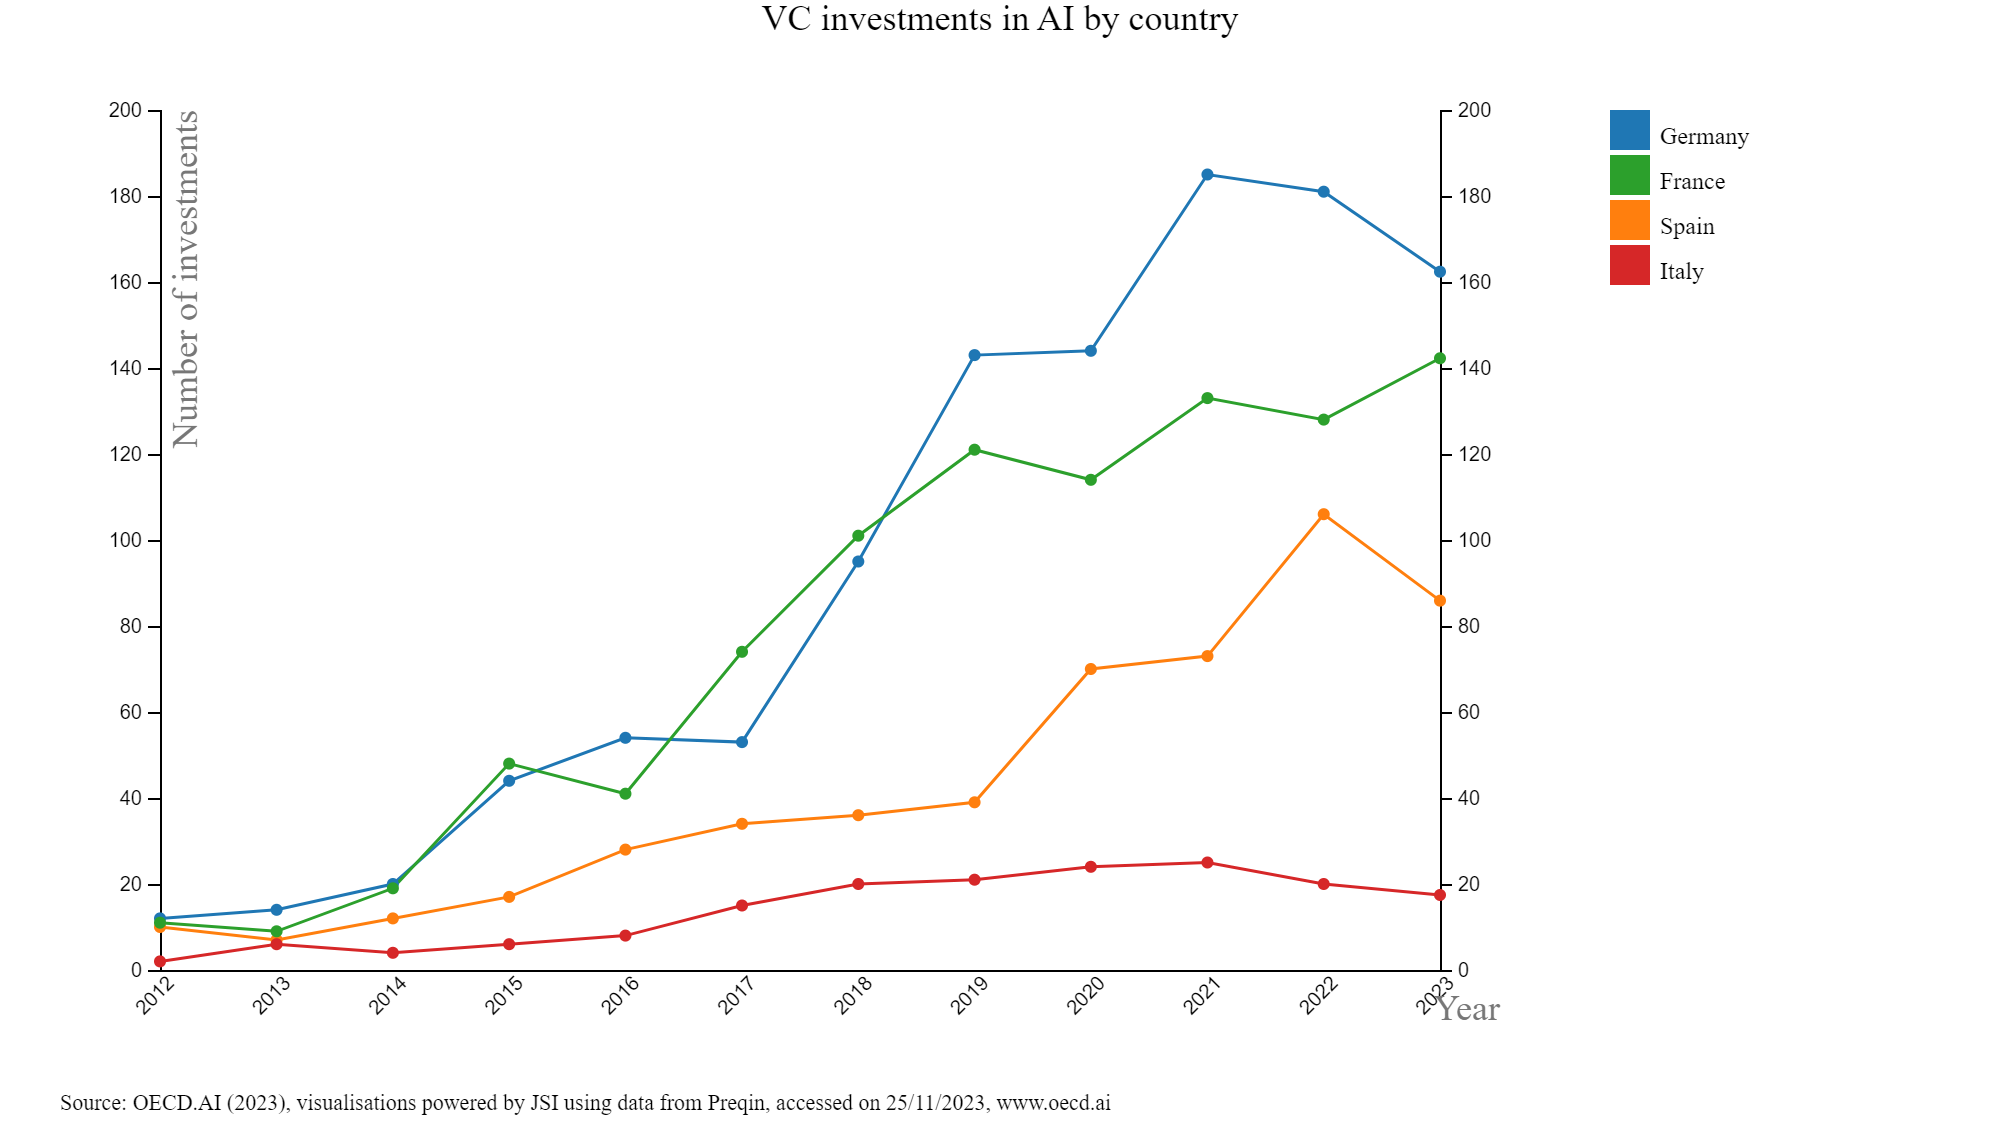
\includegraphics[width=0.3\linewidth]{Numero investimenti.png}
\end{center}
\begin{justify}
    Questo grafico rappresenta il numero degli investimenti effettuati per Stato nel settore AI e Data.
\end{justify}

\begin{center}
    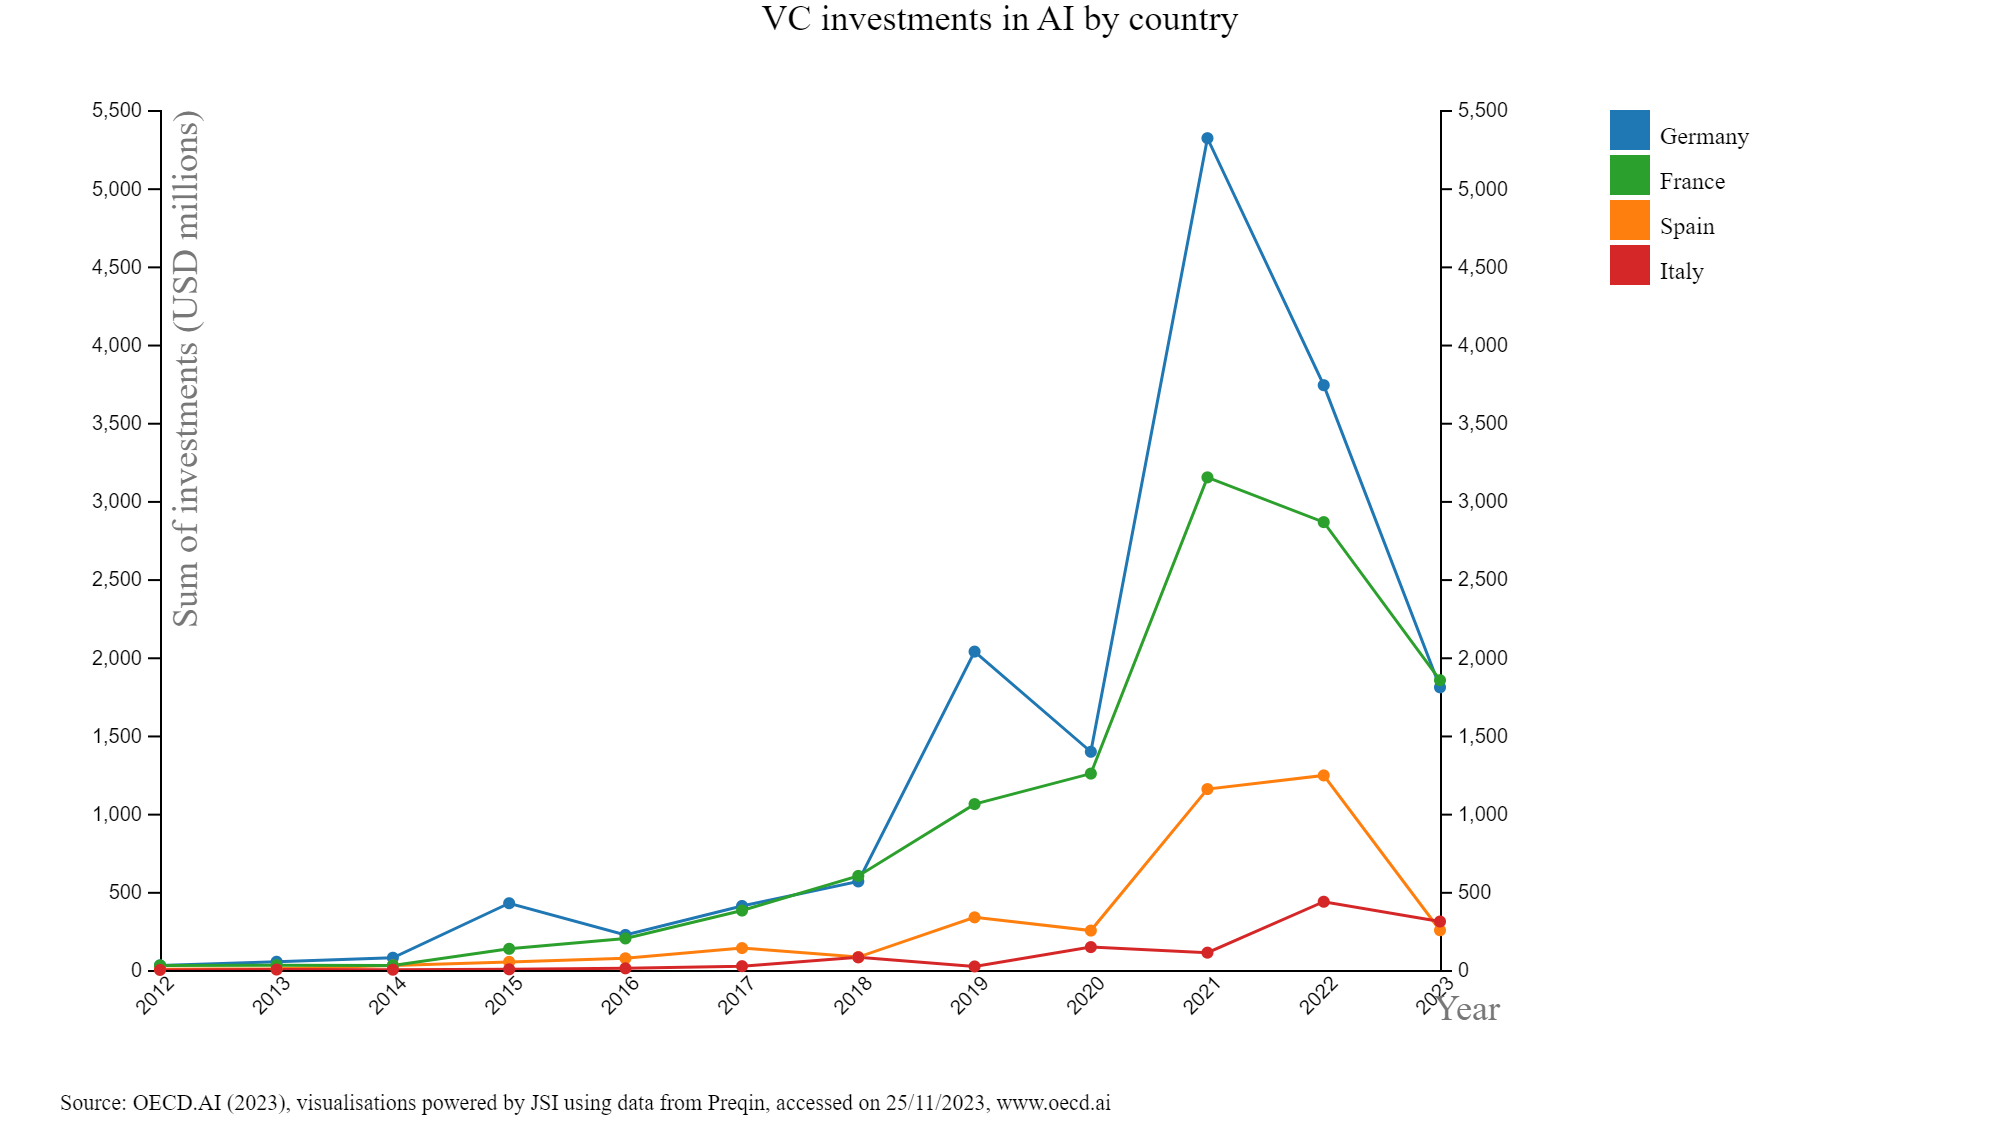
\includegraphics[width=0.3\linewidth]{Somma degli investimenti.png}
\end{center}
\begin{justify}
    Questo invece lo rappresenta sulla base dei milioni di dollari spesi in questo settore.
\end{justify}

\newpage \centering
\section{Conclusioni e opinioni finali}
\begin{justify}
   Credo che quello di cui abbiamo bisogno oggi è più conoscenza, e più dibattito pubblico, sull'intelligenza artificiale. Esiste davvero un confine netto tra umano e artificiale? L’intelligenza artificiale ci ruberà davvero il lavoro? Che impatto ambientale produce lo sviluppo e l'impiego di sistemi di IA? E cosa prevedono le norme che si stanno mettendo a punto a livello europeo?
\end{justify}
\begin{justify}
    \bibliography{Bibliografia}
    \bibliographystyle{plainnat}
\end{justify}

\end{document}